\section{Evaluation}
\label{sec:eval}


This section reports on our extensive evaluation of \SYS.
First, we present our evaluation settings.
Then, we describe the real-world dataset used in our macrobenchmark experiments.
We then dig into a set of microbenchmarks that show the overhead of running the LuaVM inside the SGX enclaves.
Finally, we deploy a full \SYS pipeline, scaling the number of workers per stage, to study the limits of the system in terms of throughput and scalability.


\subsection{Evaluation settings.}
We have experimented on machines using a processor Intel$^{\tiny{\textregistered}}$~Core\texttrademark~i7-6700~\cite{intel:i7_6700} and 8GB RAM.
We use a cluster of 2 machines based on Ubuntu 14.04.1 LTS (kernel 4.2.0-42-generic).
The choice of the Linux distribution is driven by compatibility reasons with the latest Intel SGX SDK. 
The machines run Docker (v.1.13.0).
Nodes join a Docker Swarm~\cite{docker:swarm_2016} (v1.2.5) using the Consul~\cite{consul} (v0.5.2) discovery service.
The Swarm manager and the discovery service are deployed on a distinct machine.
Containers leverage the Docker overlay network to communicate to each other.
Machines are interconnected using a switched 1~Gbps network.

%\vs{add SGX things}
%\ah{in SGX things, explain the choice of Ubuntu 14.04.1}
%\ah{should we reference public repositories and specific version (commit hashes) of used stuff (driver, platform) for SGX?}


\subsection{Dataset.}
In our experiments, we process a real dataset released by the \emph{American Bureau of Transportation Statistic}~\cite{rita:bts}.
The dataset reports on the flight departures and arrivals of 20 air carriers~\cite{statistical_computing:data}.
We implement a benchmark application atop of \SYS to compute average delays and the total of delayed flights for each air carrier.
We design and implement the full processing pipeline, that (i) parses the input datasets (in a comma-separated-value format) to data structure (\textsf{map}), (ii) filters data by relevancy (\emph{i.e.}, if the data concerns a delayed flight), and (iii) finally reduces it to compute the wanted informations.\footnote{This experiment is inspired by Kevin Webber's blog entry \emph{Diving into Akka Streams}: \url{https://blog.redelastic.com/diving-into-akka-streams-2770b3aeabb0}.}
We use the 4 last years of the available dataset (from 2005 to 2008), for a total of 28 millions of entries to process and 2.73 GB of data.
%\vs{Update with the details of other datasets if any}
%\ah{wouldn't it be more logical to puts Dataset section after Micro-Benchmark one?}

\vs{stopped here}
\subsection{Micro-Benchmark: Lua in SGX.}
To estimate the cost of enclaved function calls we averaged the time it took to do one milion calls with no data transfers.
While normal function calls took 23.6 $ns$, enclaved calls took on average 2.35 $\mu s$, \textit{i.e}., two orders of magnitude worse.
We then assessed the cost of copying data from the unshielded execution to the enclave and compared with the time it took to natively do the same.
We initialized a buffer of 100 MB with random data and copied its content by chunks of increasing sizes, with one function call per chunk.
Figure~\ref{fig:sgxmemcpy} shows the results.
When using smaller chunks, the function call overhead plays an important role in the total time, which steadly drops until we send chunks of 64 KB (vertical line).
We can also notice that copying data back to non-sgx execution impose an overhead of at most 20\% when compared to the one-way copy.
Each point in the plot corresponds to the average of 20 runs. Correctness of the copies was verified by SHA256 digest comparison between reproduced memory areas.

\begin{figure}[t!]
  \centering
  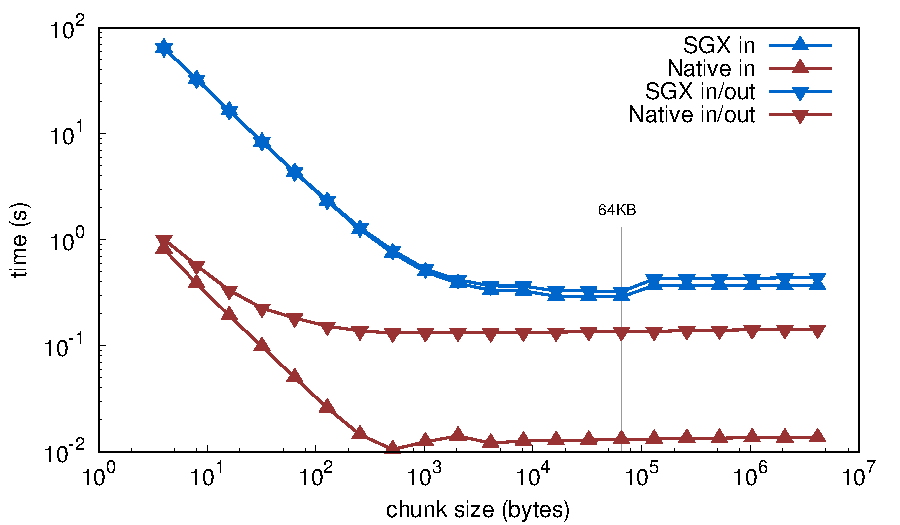
\includegraphics[scale=0.45]{plots/memcpy/memcpy.pdf}
  \caption{Time to copy 100 MB of memory}
  \label{fig:sgxmemcpy}
\end{figure}

Then we moved to the assessment of Lua benchmarks.
We chose six out of the eleven available in a standard set of benchmarks \cite{bolz2015} based on their dependency on input/output instructions.
We ran each benchmark twenty times with the same pair of parameters as originally published, both in our SGX Lua interpreter and natively at the same machine.
Results are shown in Figure~\ref{fig:luabenchs}.
Since the whole memory area has to be previously allocated in the current version of SGX and our biggest test used more than 600~MB of memory, wall clock time comparison would not be equitative for smaller tests.
In such cases, almost the whole execution time is dedicated to memory allocation.
Because of that, we subtracted the allocation time from the measurements of enclave executions, based on the average for the 20 runs.
Fluctuations on this measurement caused the apparent effect of SGX executions being faster than native ones (by at most 3\%), which is obviously non realistic.
Table~\ref{tab:luabmarks} lists the parameters along with the maximum used amount of memory and the ratio between runtimes of sgx and native executions.
Whenever the memory usage is kept low, the performance overhead is not high (less than 15\% in our experiments). When the amount of memory usage rises, however, performance drops to almost 5 times worse, as for the \emph{binarytrees} experiment.

\begin{figure}[b!]
  \centering
  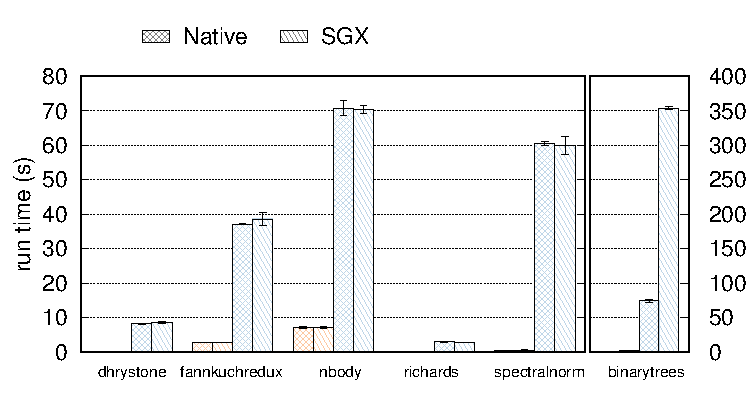
\includegraphics[scale=0.65]{plots/microbenchmark_luasgx/microbenchmark_luasgx.pdf}
  \caption{Enclave versus native running times for Lua benchmarks}
  \label{fig:luabenchs}
\end{figure}

\newcommand{\higparamcolor}{\rowcolor[rgb]{0.79,0.91,0.90}\cellcolor{white}}
\newcommand{\lowparamcolor}{\rowcolor[rgb]{0.94,0.88,0.76}\cellcolor{white}}
\begin{table}[h!]
    \centering
    \begin{tabular}{|c|c|c|c|}
    \hline
               &parameter  &memory      &ratio \\
               &           &peak        &sgx/native \\
    \hline
\lowparamcolor
dhrystone      &50K        &275KB       & 1.14 \\
\higparamcolor
               &5M         &275KB       & 1.04 \\
    \hline
\lowparamcolor
fannkuchredux  &10         &28KB        & 0.99 \\
\higparamcolor
               &11         &28KB        & 1.04 \\
    \hline
\lowparamcolor
nbody          &2.5M       &38KB        & 0.99 \\
\higparamcolor
               &25M        &38KB        & 1.00 \\
    \hline
\lowparamcolor
richards       &10         &106KB       & 1.02 \\
\higparamcolor
               &100        &191KB       & 0.97 \\
    \hline
\lowparamcolor
spectralnorm   &500        &52KB        & 1.00 \\
\higparamcolor
               &5K         &404KB       & 0.99 \\
    \hline
\lowparamcolor
binarytrees    &14         &25MB        & 1.18 \\
\higparamcolor
               &19         &664MB       & 4.76 \\
    \hline
    \end{tabular}
    \caption{\label{tab:luabmarks}Parameters and memory usage for Lua benchmarks}
\end{table}

\subsection{Benchmark: throughput.}
This benchmark shows the upload throughput observed across the whole cluster while streaming the dataset as fast as possible from the source nodes into the processing pipeline.
We gather bandwidth measurements by exploiting Docker's own monitoring and statistical module.
%Throughput accross containers wrapping each node of the processing pipeline are measured from Docker stats.
The statistics are gathered at runtime while the experiment is executing.
%During the experiment, we retrieve all the data stats for each container.
%In particular, \texttt{txbytes} stats are extracted to measure containers output throughput.
We report on our results in Figure~\ref{fig:throughput}.
In this scenario, 4 nodes concurrently inject the input dataset into the processing pipeline, each one using a subset of the full dataset.
However, only one worker process is used for each step of the processing pipeline.
We use a representation based on stacked percentiles.
The white bar at the bottom represents the minimum value, the pale grey on top the maximal value.
Intermediate shades of grey represent the 25th, 50th–, median–, and 75th percentiles.
For instance, the median throughput at 200\,seconds into the experiment almost hits 2,500\,kB/s, meaning that 50\,\% of the nodes in that moment are outputting data at 2,500\,kB/s or less.
%These datas are computed to be plotted together by percentile, as shown on figure \ref{fig:throughput}.\ah{maybe it could be relevant to put three plots, corresponding to experiments 4-datas-1-worker, 4-datas-2-workers and 4-datas-4-workers}
With the current implementation, we observe a peak of 10\,MB/s upload throughput into the processing stages.%\vs{for the future, it'd be interesting to know which stage is the fastest one}
%\ah{I gonna measure throuput between two containers run on a swarm cluster, using iperf, for comparison purpose}


\vs{We should then extend this section to present how the TPUT is affected by having few/all streams going through the enclaves. This would be an interesting/useful plot as it provides useful insights.}


\subsection{Benchmark: scalability.} We conclude this preliminary by presenting scalability results of the \SYS framework.
In particular, we scale up each stage of the processing pipeline, up to 4\,workers per stage.
For each of the configurations, the experiment is repeated 20\,times.
We show average and standard deviation of the overall completion time to process the full dataset.
Figure~\ref{fig:scalability} depicts these results.
%Scalability of \SYS is evaluated by processing these datas 20 times on 3 different pipeline topology: using 1, 2 or 4 workers for each step of the pipeline.
We observe that by doubling the number of workers from the initial configuration achieves a 2$\times$ speed-up of the overall processing time, that is from 20\,minutes to less than 10\,minutes.
Conversely, we do not observe similar improvements when using 4\,workers.
%Results are represented on figure \ref{fig:scalability}, and show clearly better performances between the experiment using only one worker by task, and the one using 2 workers.
%In an other hand, using 4 workers instead of 2 does not show any performance improvement.

\begin{figure}[t!]
  \centering
  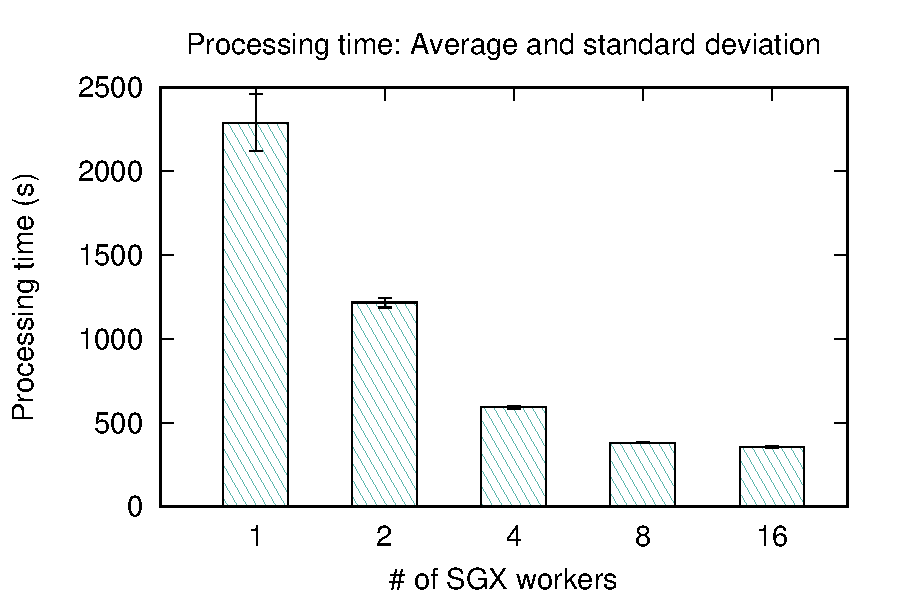
\includegraphics[scale=0.5]{plots/secure_streams/scalability/sgxmapper_scalability.pdf}
  \caption{Scalability: processing time, average and standard deviation. The experiment is repeated 5 times, with a variation on the number of mappers SGX, other workers - 1 filter worker and 1 reduce worker - do not use SGX.}
  \label{fig:scalability}
\end{figure}

We believe this behavior can be explained by existing bottlenecks in the pipelining infrastructure, lack of optimization in the application logic as well as tuning options of the \zmq queues.
These hypotheses are confirmed by observing the throughput of the system once we increase the processing workers to 2 and 4 in Figure~\ref{fig:throughput2} and Figure~\ref{fig:throughput4}, respectively.
We observe the following facts.
First, the system is far from saturating the network's available bandwidth, hitting a peak of 10\,MB/s.
Second, a small percentage of nodes consumes much more bandwidth than the other components.
We intend to further investigate these effects as part of our future work, as we are going to elaborate in the following section.


\begin{figure*}[!t]
\centering
\begin{tabular}{cccc}
\subfloat[Throughput without encoding]{
  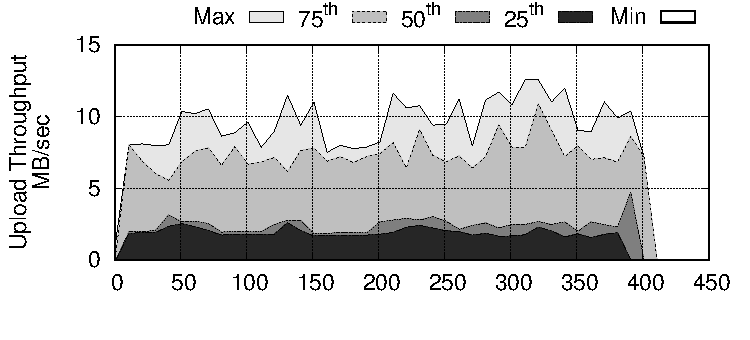
\includegraphics[width=.31\linewidth]{plots/secure_streams/throughput/tput_tx_percentiles_1-workers}
} &
\subfloat[Throughput without SGX]{
  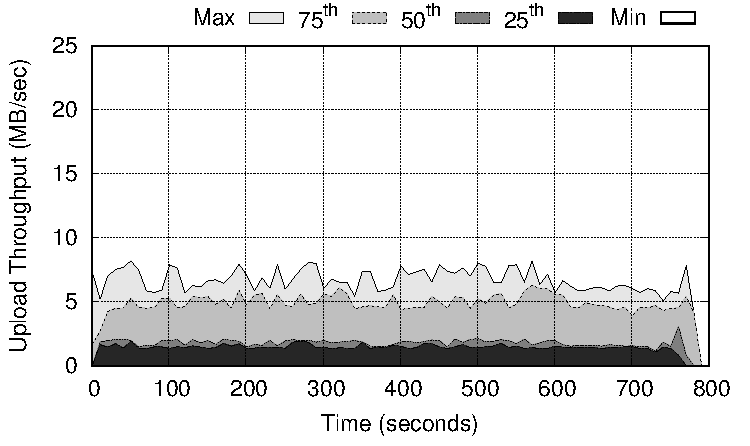
\includegraphics[width=.31\linewidth]{plots/secure_streams/throughput/tput_tx_percentiles_1-workers-encrypted-nosgx}
} &
\subfloat[Throughput with SGX]{
  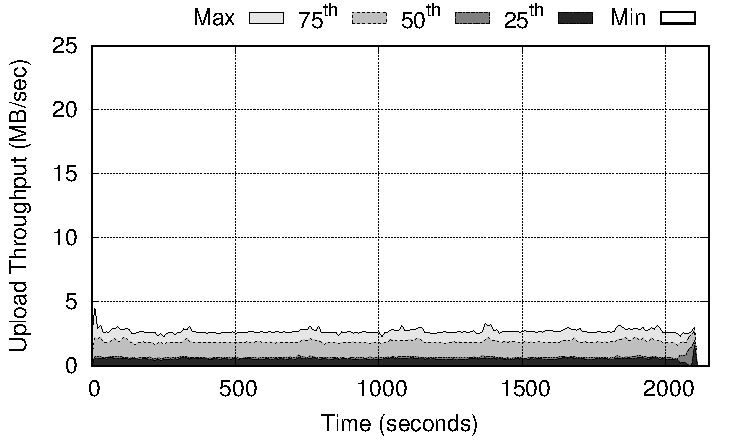
\includegraphics[width=.31\linewidth]{plots/secure_streams/throughput/tput_tx_percentiles_1-workers-encrypted-fullsgx}
}\cr
\subfloat[Throughput without encoding]{
  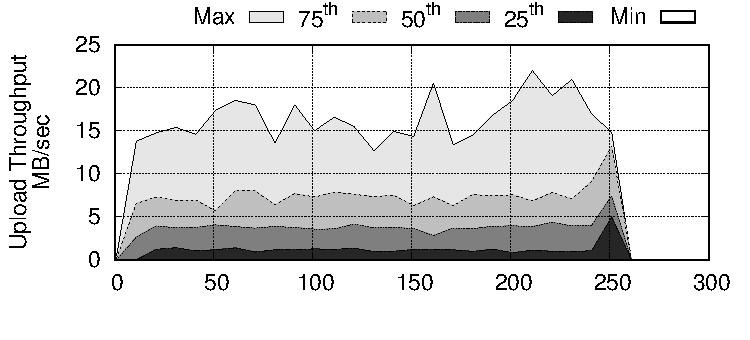
\includegraphics[width=.31\linewidth]{plots/secure_streams/throughput/tput_tx_percentiles_2-workers}
} &
\subfloat[Throughput without SGX]{
  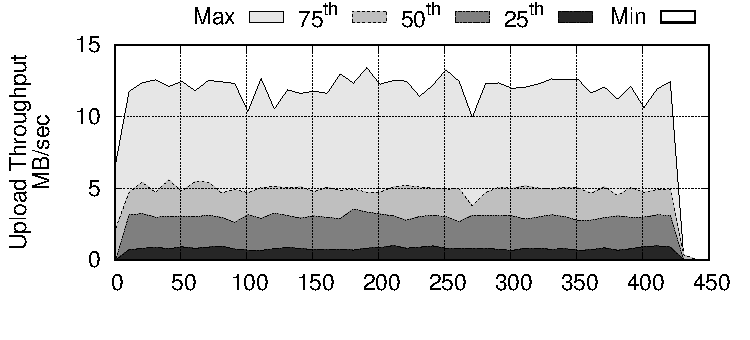
\includegraphics[width=.31\linewidth]{plots/secure_streams/throughput/tput_tx_percentiles_2-workers-encrypted-nosgx}
} &
\subfloat[Throughput with SGX]{
  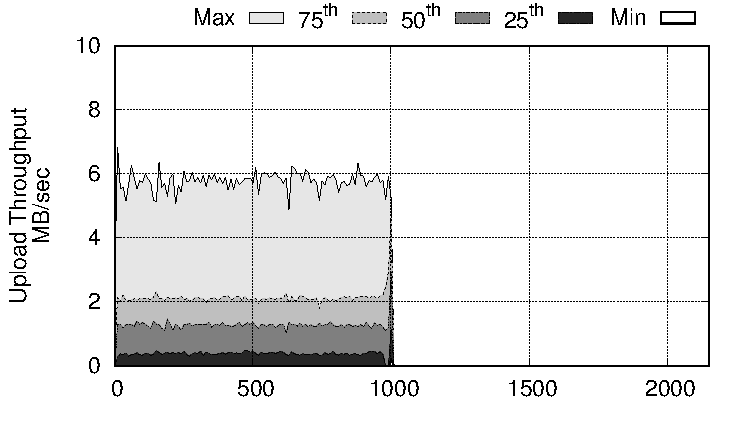
\includegraphics[width=.31\linewidth]{plots/secure_streams/throughput/tput_tx_percentiles_2-workers-encrypted-fullsgx}
}\cr
\subfloat[Throughput without encoding]{
  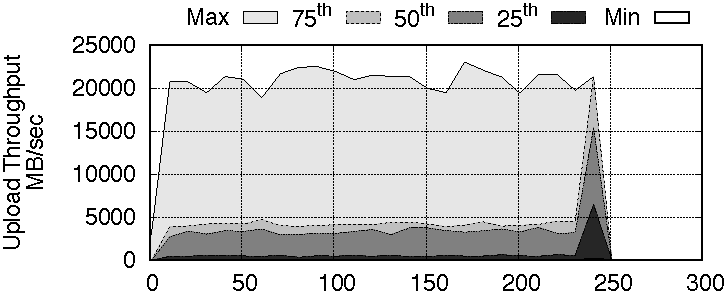
\includegraphics[width=.31\linewidth]{plots/secure_streams/throughput/tput_tx_percentiles_4-workers}
} &
\subfloat[Throughput without SGX]{
  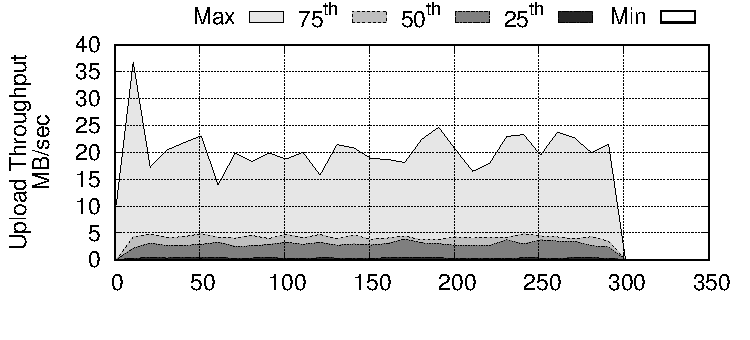
\includegraphics[width=.31\linewidth]{plots/secure_streams/throughput/tput_tx_percentiles_4-workers-encrypted-nosgx}
} &
\subfloat[Throughput with SGX]{
  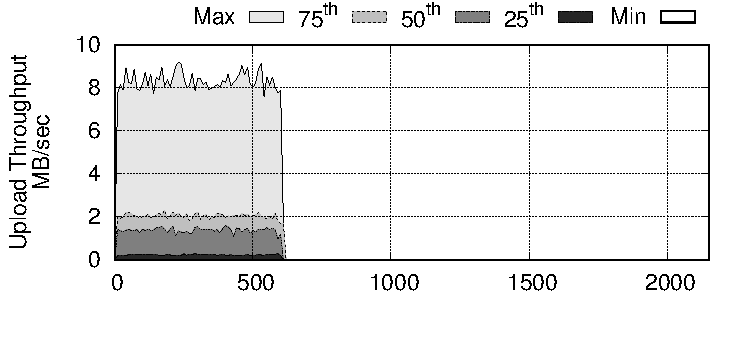
\includegraphics[width=.31\linewidth]{plots/secure_streams/throughput/tput_tx_percentiles_4-workers-encrypted-fullsgx}
}
\end{tabular}
\caption{Throughput comparison between normal processing and SGX processing}
\end{figure*}

